\documentclass[12pt]{article}

\usepackage[margin=1.0in]{geometry}
\usepackage{hyperref}
\usepackage{graphicx}
\usepackage{multicol}
\usepackage{subcaption}
\usepackage{parskip}
\usepackage[title,toc]{appendix}
\usepackage{enumerate}
\usepackage{amsmath}
\usepackage{fancyhdr}
\usepackage{setspace}

\captionsetup[sub]{font=footnotesize}

\hypersetup
{
	colorlinks,
	linkcolor = black,
	urlcolor = black,
	citecolor = black
}

\usepackage{booktabs}
\usepackage{array}
\newcolumntype{R}{>{\raggedleft\arraybackslash}p{1cm}}

\usepackage{apacite}
\bibliographystyle{apacite}

%\usepackage{natbib}

%\renewcommand{\bibsection}{\chapter*{\refname}}

\pagestyle{fancy}

\lhead{Acma 490 Project}
\rhead{Nathan Esau}

\title{Acma 490 Project}
\author{Nathan Esau}
\date{Spring 2017}

\begin{document}
\nocite{*}

\maketitle

\tableofcontents

\newpage

\section{Executive Summary}

This report details the findings regarding the new endowment insurance product your company is considering to launch. This non-taxable product should be attractive to wealthy investors (who may have used their max TFSA or RRSP room already) for two reasons:

\begin{enumerate}[(i)]
\item If the policyholder dies during the contract term, they get a substantial death benefit (between \$500,000 to \$5,000,000).
\item If the policyholder survives the contract term they will typically earn a positive return on their premium (up to 7.5\% depending on their age and the term of the product). Furthermore, this return is not taxable.
\end{enumerate}

This report assumed that investors want the highest survival benefit possible in relation to their death benefit. For example, a female policyholder aged 30 would prefer \$25,000 of survival benefit to \$20,000 when the death benefit is \$1,000,000. The rationale is that investors hope to earn a positive, non-taxable return should they survive the contract term.

In order to satisfy the regulation such that the product is classified as insurance, the death benefit must be significantly larger than the survival benefit (for most ages). For instance, a female policyholder aged 30 would require a death benefit around 40 times larger than their survival benefit. 

This makes the insurance risk much higher for young ages. For instance, a female policyholder aged 30 would pay around \$20,000 for a 10-year product with \$1,000,000 of death benefit and \$25,000 of survival benefit. If the policyholder dies, there is a massive loss for the insurer. It is possible for this type of risk to be mitigated through pooling.

Longer term contracts have less mortality risk, but more investment risk. The rationale is that we are likely to pay the survival benefit, but we are uncertain about the return earned over long periods.

Investment risk could be reduced by selling shorter-term contracts, but this would create more insurance risk. However, investors are likely to demand 10 year contracts since they lead to higher returns for the survival benefit so it may be necessary to offer these contacts. If the investment risk is a still a concern, a safer investment strategy could be considered. However, if this were done investors would need to be charged a higher premium making the product less competitive.

The pricing was done quite conservatively -- an Ornstein-Uhlenbeck process with 5\% long-term mean was used to model returns, whereas historical company returns have consistently been above 5\%. Should investments continue to perform as well as they have historically, the charged premium is higher than needed which would lead to insurer profits.

The analysis in this report revealed that with 2000 policies, the standard deviation per policy is around 8\% of the premium. About 9\% of this risk is coming from mortality risk and 91\% is coming from investment risk. Using a benchmark standard deviation of 10\% of premium as ``acceptable'' this product is feasible to sell in the market since the standard deviation per dollar premium is only 8\%.

\section{Assumptions}

\subsection{Interest Rate}

The interest rate was modeled by an Ornstein-Uhlenbeck process. Parameters were estimated using historical company returns from the past 5 years (monthly observation frequency, annualized returns). A long-term rate of 5\% was assumed.

The least-squares method gave a AR(1) process with $\phi_{1} = 0.9793$, $\sigma_{2} =  0.00372$, $\delta_{0} = 0.0767$ and $\delta = 0.05$. This is equivalent to an OU process with $\delta_{0} = 0.0767$, $\delta = 0.05$, $\alpha = 0.2506$ and $\sigma = 0.01302$.

A forecast of the future interest rate is shown in Figure \ref{fig:ouforecast}. An OU process fit to historical returns from 1991 to 2017 is shown in Appendix A.1.

\begin{figure}[ht]
\begin{center}
\vspace{-12.5mm}
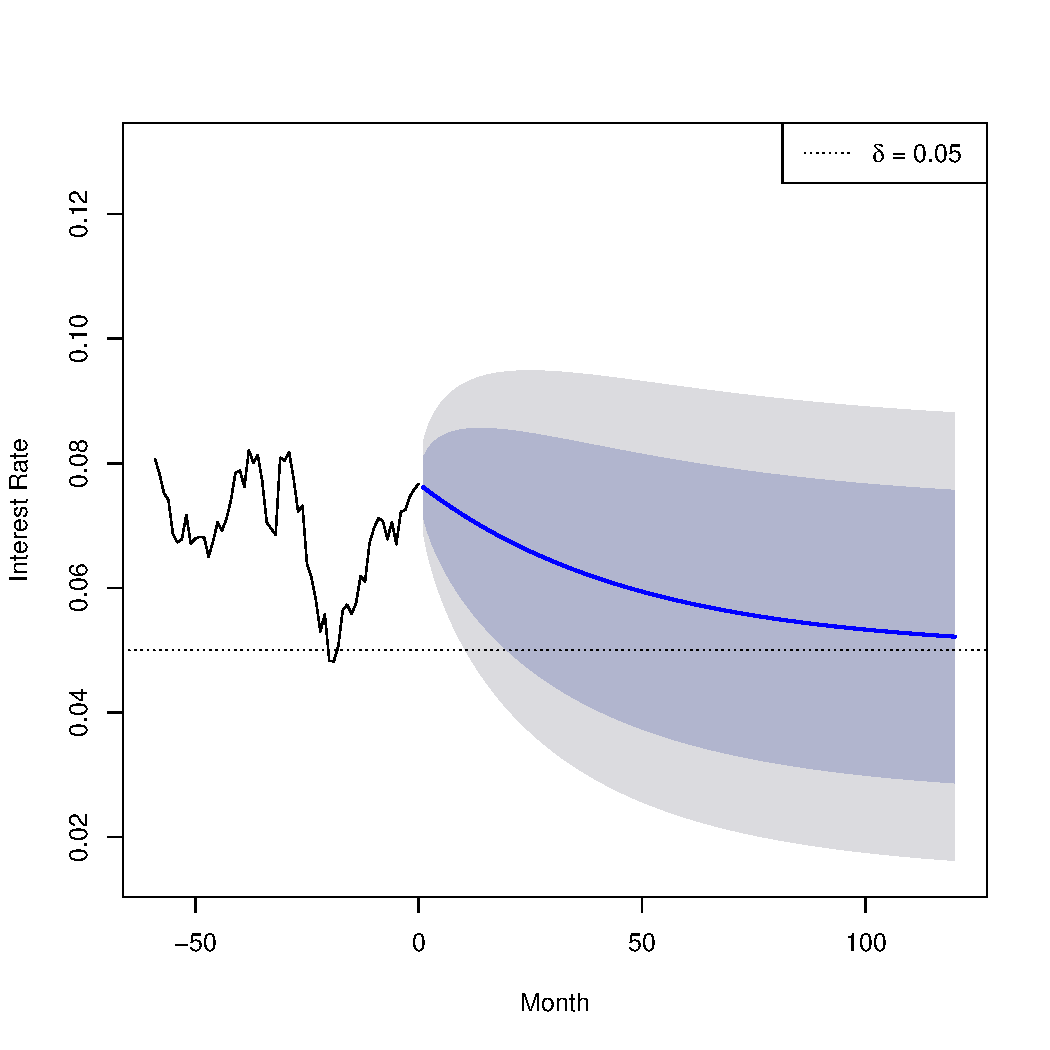
\includegraphics[width=0.75\textwidth]{images/arforecast}
\end{center}
\caption{Expected interest rate over next 10 years using an OU process with $\delta_{0} = 0.0767$, $\delta = 0.05$, $\alpha = 0.2506$ and $\sigma = 0.01302$. The 80\% and 95\% confidence intervals are shown.}
\label{fig:ouforecast}
\end{figure}

It is worth mentioning that historical returns have been much higher than 5\% as shown in Appendix A.1. Pricing at a 5\% interest rate leads to a higher premium than if the historical average return were used.

\subsection{Mortality}

The 1991 Canadian Life Table was used. Male and Female policyholders were analyzed separately since they have quite different mortality for older ages. This is demonstrated in Figure \ref{fig:curvedeaths}.

\begin{figure}[ht]
\begin{center}
\vspace{-12.5mm}
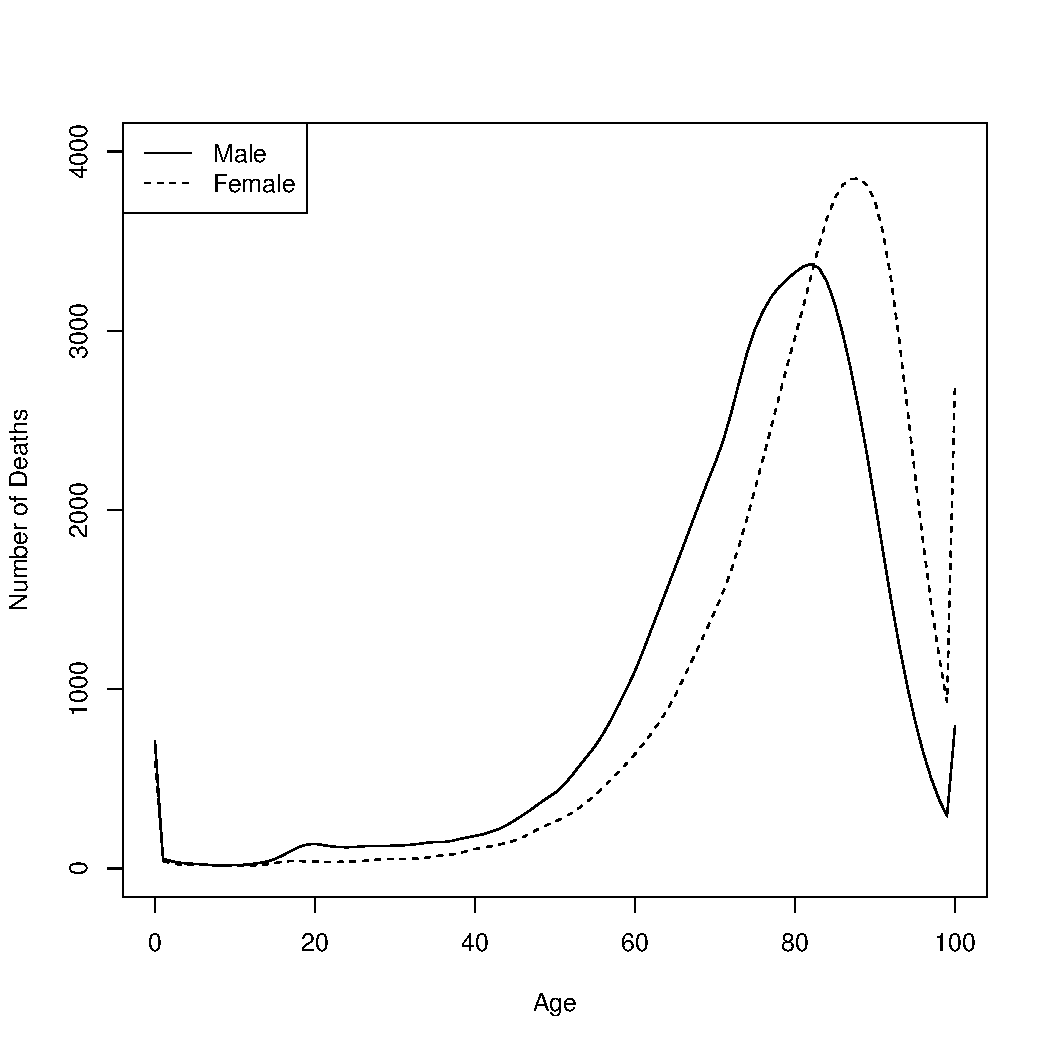
\includegraphics[width=0.75\textwidth]{images/curvedeaths}
\end{center}
\vspace{-2.5mm}
\caption{Curves of deaths for 100,000 newborns based on 1991 Canadian life table}
\label{fig:curvedeaths}
\end{figure}

\subsection{Age Distribution}

It was assumed that policyholders range in age from 25 to 75, with the most policyholders in the age intervals 45-49 and 50-54.

This makes sense from a practical standpoint. This product is targeted towards wealthy investors. This makes it unlikely that a large number of young policyholders (who are less wealthy) would purchase this product. Those around 50 years around are looking for financial protection should they die before retirement, and investment income should they survive. The mode of the population is around age 50 as well (i.e. the baby boomer generation) so it makes sense that the most policyholders would be this age.

It's also unlikely that there would a large number of old policyholders because there are less old people in the population.

A histogram of the age distribution compared to the population distribution can be found in Appendix A.3.

\section{Product Analysis}

The product is a non-taxable endowment insurance with death benefit $d$ and survival benefit $e$. In this section, the risk of the product for a single policy is analyzed.

\subsection{Regulation and Pricing}

To attract investors, the survival benefit should be as large as possible. However, for the product to qualify as insurance (non-taxable) the survival benefit cannot exceed 75\% of the total benefits or 2 times the death benefit. This means that
%
\begin{align}
e = \min\left\{2, \ 3 \times \dfrac{EPV(\text{Term Insurance Contract})}{EPV(\text{Pure Endowment Contract})} \right\}
\label{eqn:endowbenefit}
\end{align}

The $EPV$ of the term insurance contract and pure endowment contract for various ages and terms can be found in Appendix A.4.

It should be pointed out that this condition on the survival benefit leads to much larger death benefits than survival benefits for the majority of ages as shown in Table \ref{tab:faceAmountTable}.

% latex table generated in R 3.3.1 by xtable 1.8-2 package
% Fri Apr 07 09:16:53 2017
\begin{table}[ht]
\centering
\begingroup\small
\begin{tabular}{|l|rrrrrr|rrrrrr|}
  \hline
& \multicolumn{6}{c|}{5-year} & \multicolumn{6}{c|}{10-year} \\
 & \multicolumn{3}{c}{Male} & \multicolumn{3}{c|}{Female} & \multicolumn{3}{c}{Male} & \multicolumn{3}{c|}{Female} \\
 \hline
Age & $d$ & $e$ & NSP & $d$ & $e$ & NSP & $d$ & $e$ & NSP & $d$ & $e$ & NSP \\ 
  \hline
25 & 1000 & 21.6 & 21.7 & 1000 & 7.8 & 7.8 & 1000 & 51.4 & 39.3 & 1000 & 19.4 & 15.0 \\ 
  30 & 1000 & 23.4 & 23.5 & 1000 & 9.4 & 9.5 & 1000 & 57.9 & 44.2 & 1000 & 25.8 & 19.8 \\ 
  35 & 1000 & 27.6 & 27.7 & 1000 & 13.7 & 13.8 & 1000 & 72.7 & 55.3 & 1000 & 39.2 & 30.1 \\ 
  40 & 1000 & 36.9 & 36.9 & 1000 & 21.6 & 21.7 & 1000 & 107.6 & 81.0 & 1000 & 62.5 & 47.6 \\ 
  45 & 1000 & 59.5 & 59.2 & 1000 & 34.5 & 34.6 & 1000 & 174.4 & 129.1 & 1000 & 100.2 & 75.6 \\ 
  50 & 1000 & 96.1 & 94.5 & 1000 & 55.3 & 55.1 & 1000 & 291.7 & 209.6 & 1000 & 163.2 & 121.2 \\ 
  55 & 1000 & 162.9 & 157.2 & 1000 & 90.5 & 89.2 & 1000 & 506.5 & 345.5 & 1000 & 264.7 & 191.5 \\ 
  60 & 1000 & 280.8 & 262.2 & 1000 & 143.9 & 139.6 & 1000 & 869.4 & 547.1 & 1000 & 430.9 & 299.4 \\ 
  65 & 1000 & 460.7 & 410.3 & 1000 & 233.9 & 221.4 & 1000 & 1474.7 & 822.3 & 1000 & 713.9 & 464.8 \\ 
  70 & 1000 & 752.0 & 622.4 & 1000 & 380.4 & 345.9 & 1000 & 2000.0 & 989.4 & 1000 & 1252.4 & 727.8 \\ 
  75 & 1000 & 1295.3 & 948.7 & 1000 & 668.6 & 564.7 & 1000 & 2000.0 & 928.5 & 1000 & 2000.0 & 995.9 \\ 
   \hline
\end{tabular}
\endgroup
\caption{Net Single Premium in Thousands of Dollars for Death Benefit of \$1,000,000 and Survival Benefit satisfying the regulation. A 5\% profit and expense loading is included in the premium.} 
\label{tab:faceAmountTable}
\end{table}

.

Some of the policies are quite expensive (for instance, a 10-year contract issued to a Female aged 75 would cost \$995,900). For such a policy, the insurer is not so much concerned about the policyholder dying -- rather the risk is that the policyholder survives. Should this policyholder survive, they are guaranteed a return of 6.48\% (see Table \ref{tab:returnTable}). Having a non-taxable guaranteed return of 6.48\% is attractive to potential policyholders, but risky to offer for the insurer due to the investment risk involved.

% latex table generated in R 3.3.1 by xtable 1.8-2 package
% Fri Apr 07 09:17:01 2017
\begin{table}[ht]
\centering
\begingroup\small
\begin{tabular}{|l|rr|rr|}
  \hline
& \multicolumn{2}{c|}{5-year} & \multicolumn{2}{c|}{10-year} \\
 & \multicolumn{1}{c}{Male} & \multicolumn{1}{c|}{Female} & \multicolumn{1}{c}{Male} & \multicolumn{1}{c|}{Female} \\
 \hline
Age & Return (\%) & Return (\%) & Return (\%) & Return (\%) \\ 
  \hline
25 & -1.0868 & -1.1675 & 2.1953 & 2.1139 \\ 
  30 & -1.0760 & -1.1581 & 2.2132 & 2.1314 \\ 
  35 & -1.0510 & -1.1325 & 2.2533 & 2.1675 \\ 
  40 & -0.9959 & -1.0858 & 2.3474 & 2.2294 \\ 
  45 & -0.8627 & -1.0087 & 2.5205 & 2.3286 \\ 
  50 & -0.6497 & -0.8874 & 2.8182 & 2.4918 \\ 
  55 & -0.2673 & -0.6825 & 3.3374 & 2.7469 \\ 
  60 & 0.3887 & -0.3772 & 4.1433 & 3.1528 \\ 
  65 & 1.3446 & 0.1294 & 5.3527 & 3.8041 \\ 
  70 & 2.8075 & 0.9254 & 6.5501 & 4.9410 \\ 
  75 & 5.2528 & 2.4031 & 7.1859 & 6.4842 \\ 
   \hline
\end{tabular}
\endgroup
\caption{Investment return on the survival benefit conditional on the policyholder surviving the term of the contract.} 
\label{tab:returnTable}
\end{table}



The risk of the term insurance component (i.e. death benefit) and pure endowment component (i.e. survival benefit) are analyzed next.

\subsection{Term Insurance Component}

The product we are offering pays a benefit of $d$ if the policyholder dies within the term of the contract.

The standard deviation per dollar premium is shown in Figure \ref{fig:sdterm}. The following observations can be made:

\begin{itemize}
\item The standard deviation per dollar premium is highest for young ages and short term contracts. This standard deviation is almost exclusively coming from the insurance risk and not the investment risk.
\item Female policyholders are less likely to die, so they pay less than male policyholders for an equivalent death benefit. This makes the standard deviation per dollar premium higher for female policyholders.
\end{itemize}

\begin{figure}[ht]
\begin{center}
\vspace{-20mm}
\centerline{
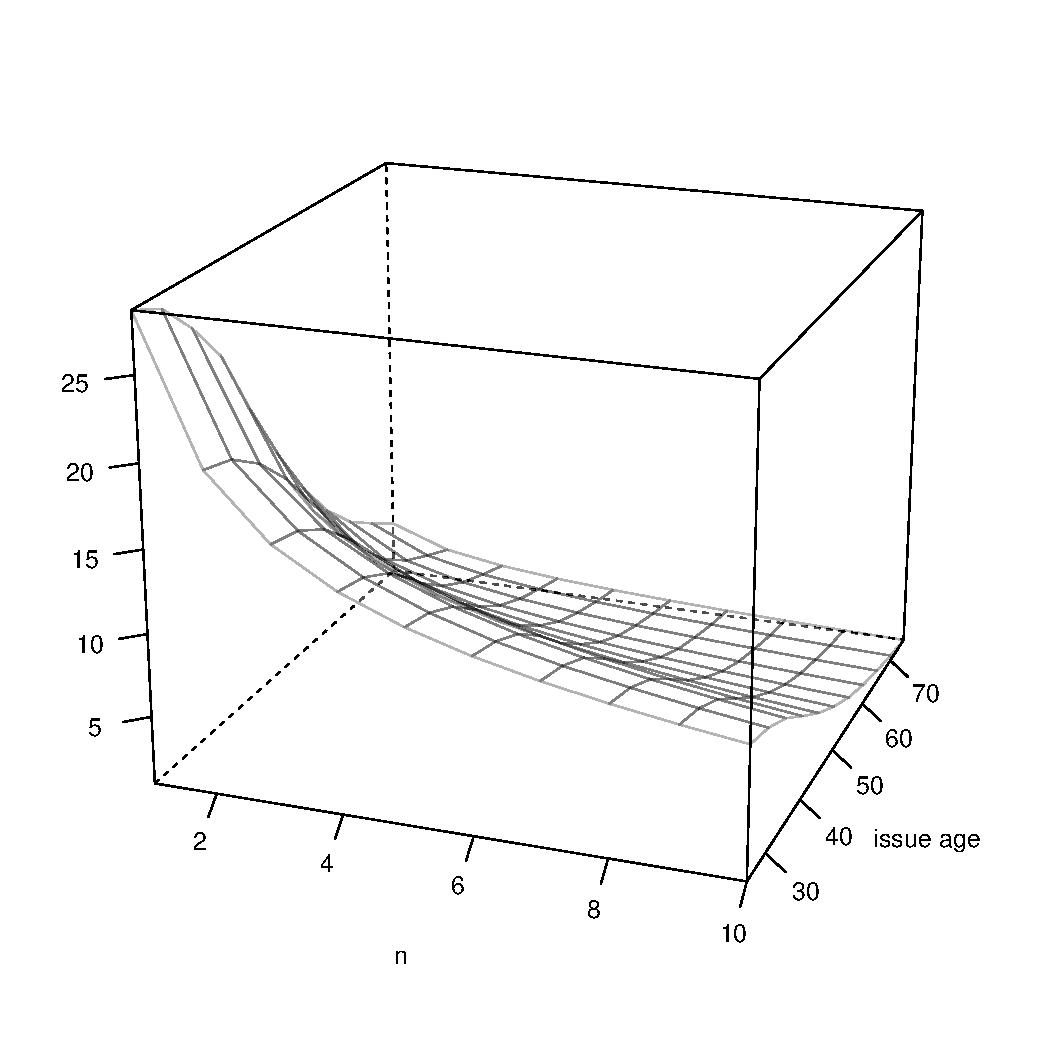
\includegraphics[width=0.6\textwidth]{images/termSDPlotMale}
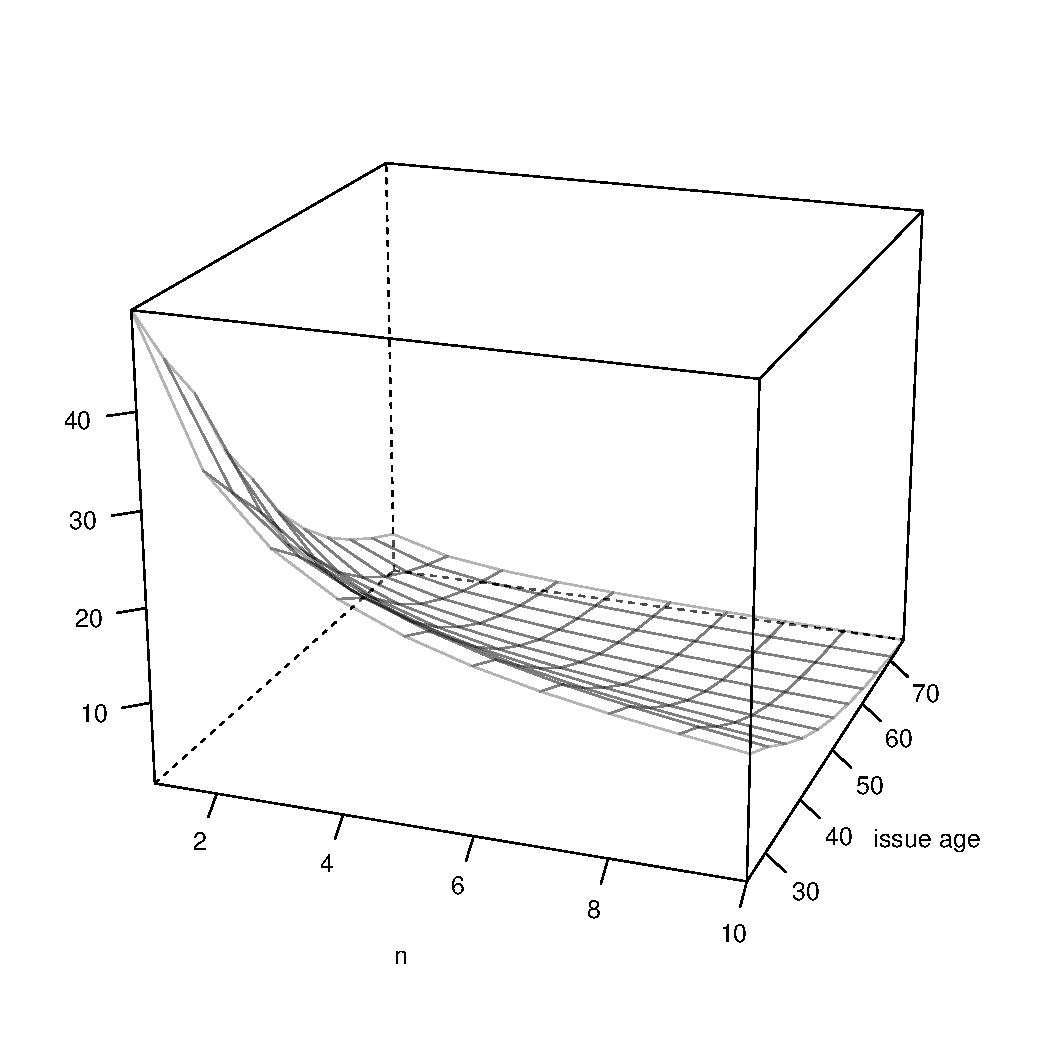
\includegraphics[width=0.6\textwidth]{images/termSDPlotFemale}}
\end{center}
\vspace{-10mm}
\caption{Standard deviation per dollar of the net single premium for $n$-year term insurance at various issue ages (male: left, female: right)}
\label{fig:sdterm}
\end{figure}

Figure \ref{fig:sdterm} highlights why pooling is necessary. Most of the risk associated with the term component can be mitigated by selling a many policies to similar ages as shown later.

\subsection{Pure endowment component}

The product we are offering pays $e$ upon survival. For the pure endowment component, the standard deviation per dollar premium is shown in Figure \ref{fig:sdpure}.

\begin{figure}[!ht]
\begin{center}
\vspace{-12mm}
\centerline{
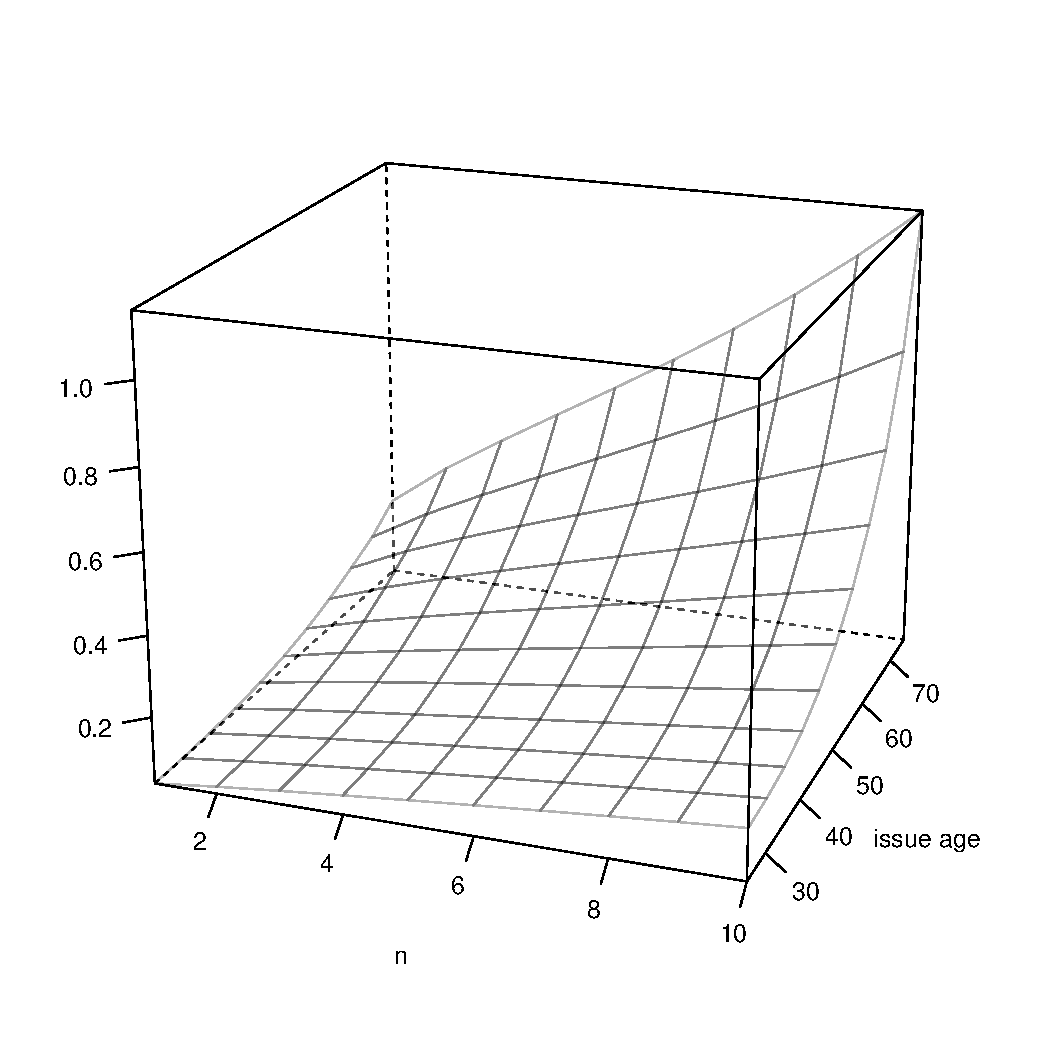
\includegraphics[width=0.6\textwidth]{images/pureSDPlotMale}
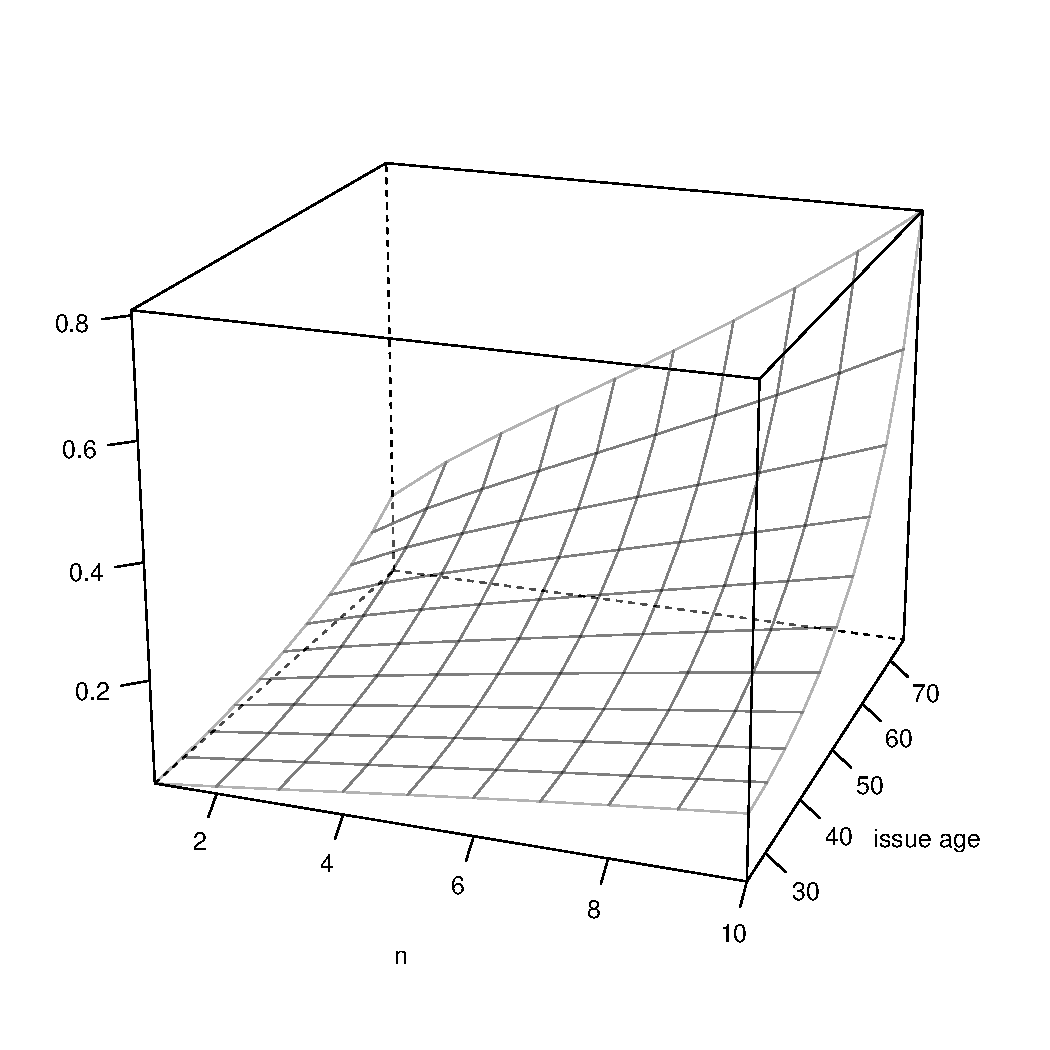
\includegraphics[width=0.6\textwidth]{images/pureSDPlotFemale}}
\end{center}
\vspace{-10mm}
\caption{Standard deviation per dollar of the net single premium for $n$-year pure endowment insurance at various issue ages (male: left, female: right)}
\label{fig:sdpure}
\end{figure}

The risk is worse for older ages, since we are unsure whether these policyholders will survive. Also, the risk is worse for longer contracts. This makes sense as the standard deviation of the present value is increasing for $n < 10$ (see Figure \ref{fig:pvvar}).

\begin{figure}[ht]
\vspace{-10mm}
\begin{center}
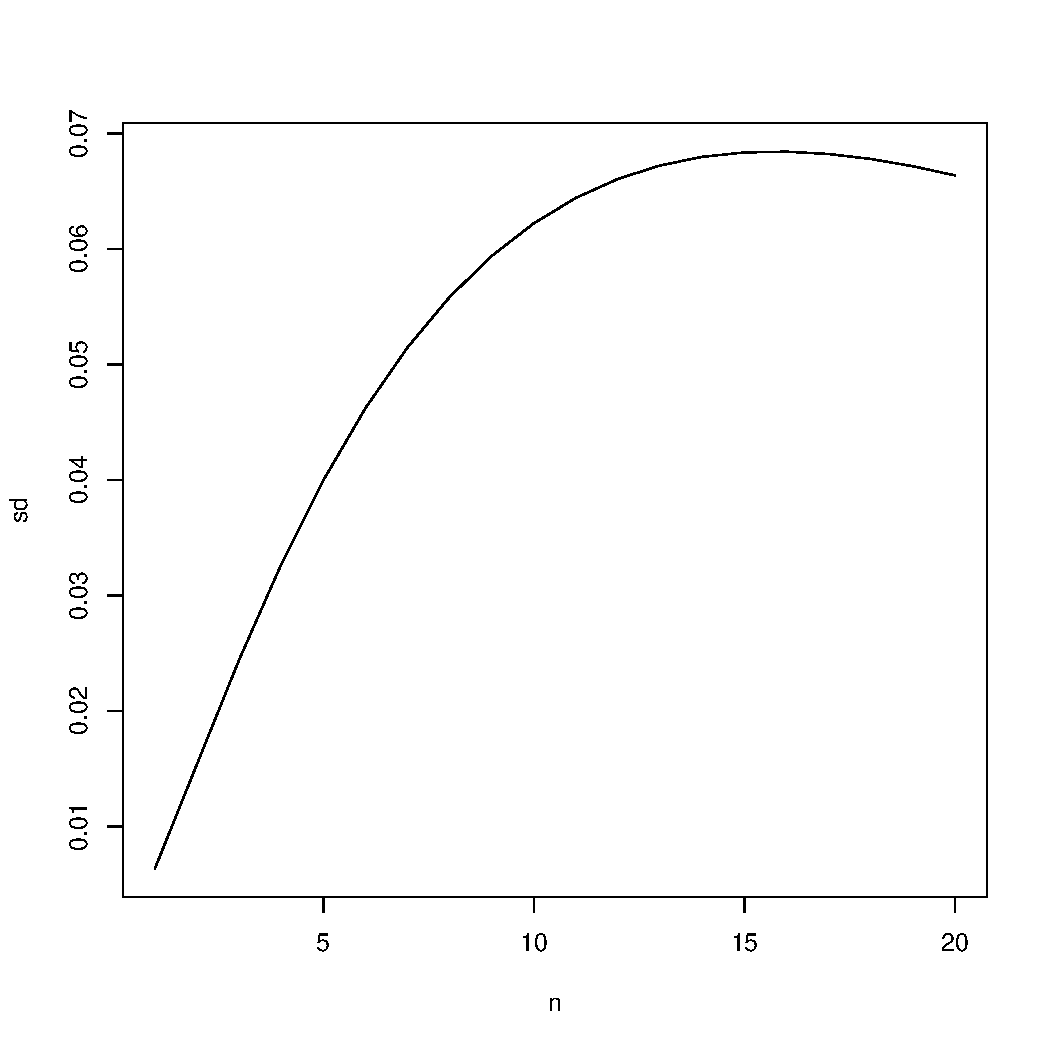
\includegraphics[width=0.55\textwidth]{images/varpv}
\vspace{-5mm}
\end{center}
\caption{Standard deviation of present value function for term $n$}
\label{fig:pvvar}
\end{figure}

\subsection{Endowment contract}

For a death benefit of $d$ and survival benefit of $e$ satisfying the regulation (i.e. using Equation \ref{eqn:endowbenefit}) we can look at the standard deviation per dollar premium. This is shown in Figure \ref{fig:sdendow}.

\begin{figure}[!htpb]
\begin{center}
\vspace{-15mm}
\centerline{
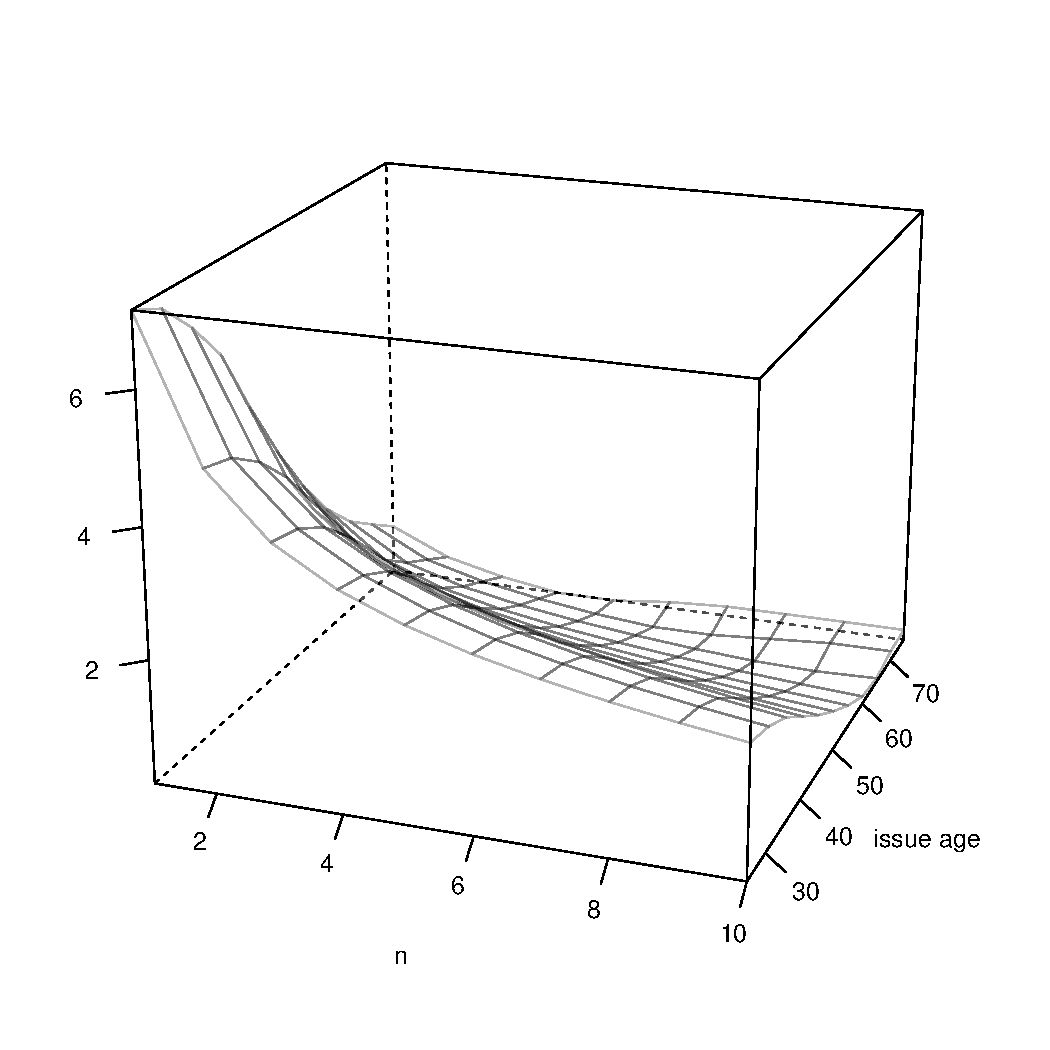
\includegraphics[width=0.6\textwidth]{images/endowSDPlotMale}
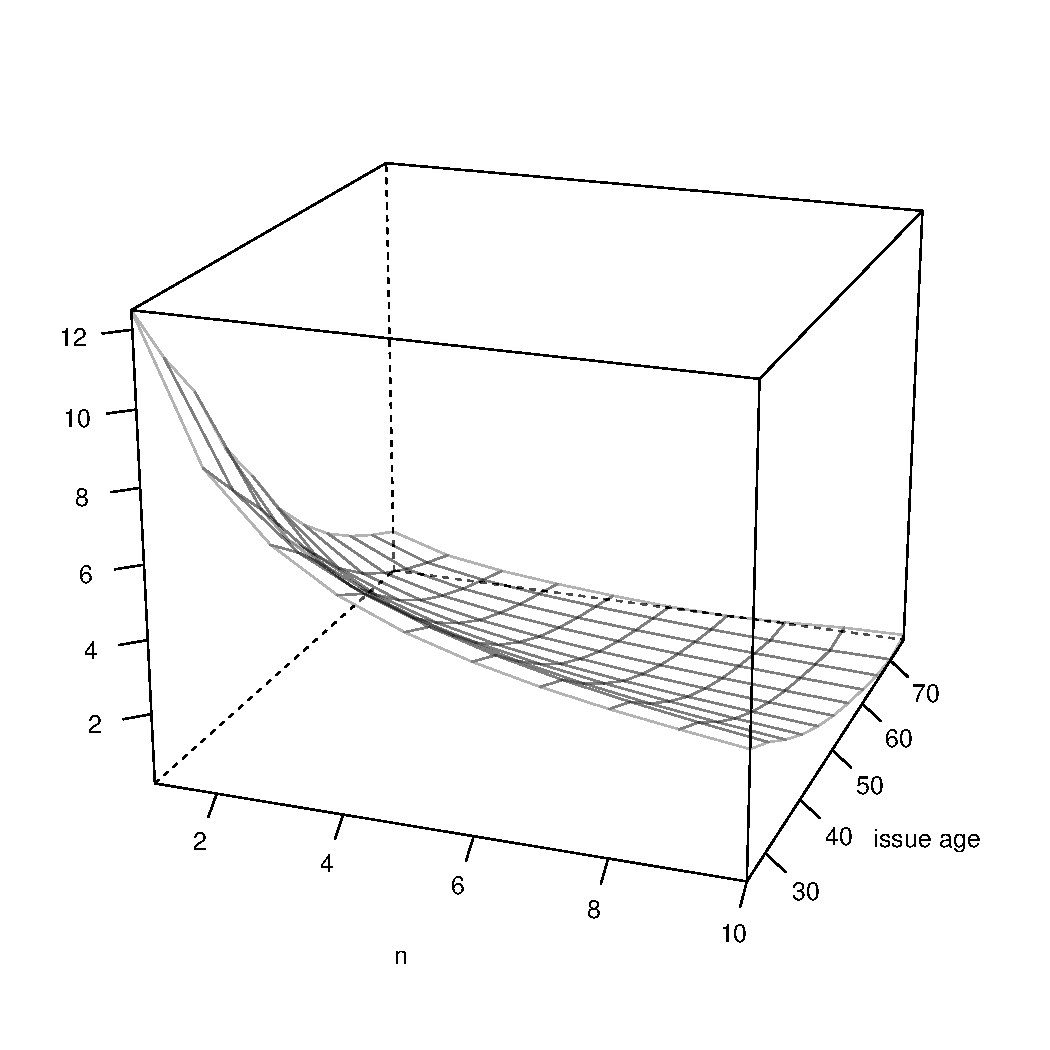
\includegraphics[width=0.6\textwidth]{images/endowSDPlotFemale}}
\end{center}
\vspace{-10mm}
\caption{Standard deviation per dollar of the net single premium for $n$-year endowment insurance at various issue ages (male: left, female: right)}
\label{fig:sdendow}
\end{figure}

We can see that the shape is very similar to that of a term insurance contract, since, to satisfy the regulation, the death benefit is far larger than the survival benefit for most ages.

\section{Portfolio of policies}

The standard deviation per dollar premium can also be analyzed for a portfolio (Figure \ref{fig:portfoliosd}).

\vspace{-11mm}
\begin{figure}[!htpb]
\begin{center}
\centerline{
\begin{minipage}[b]{0.55\textwidth}
\begin{center}
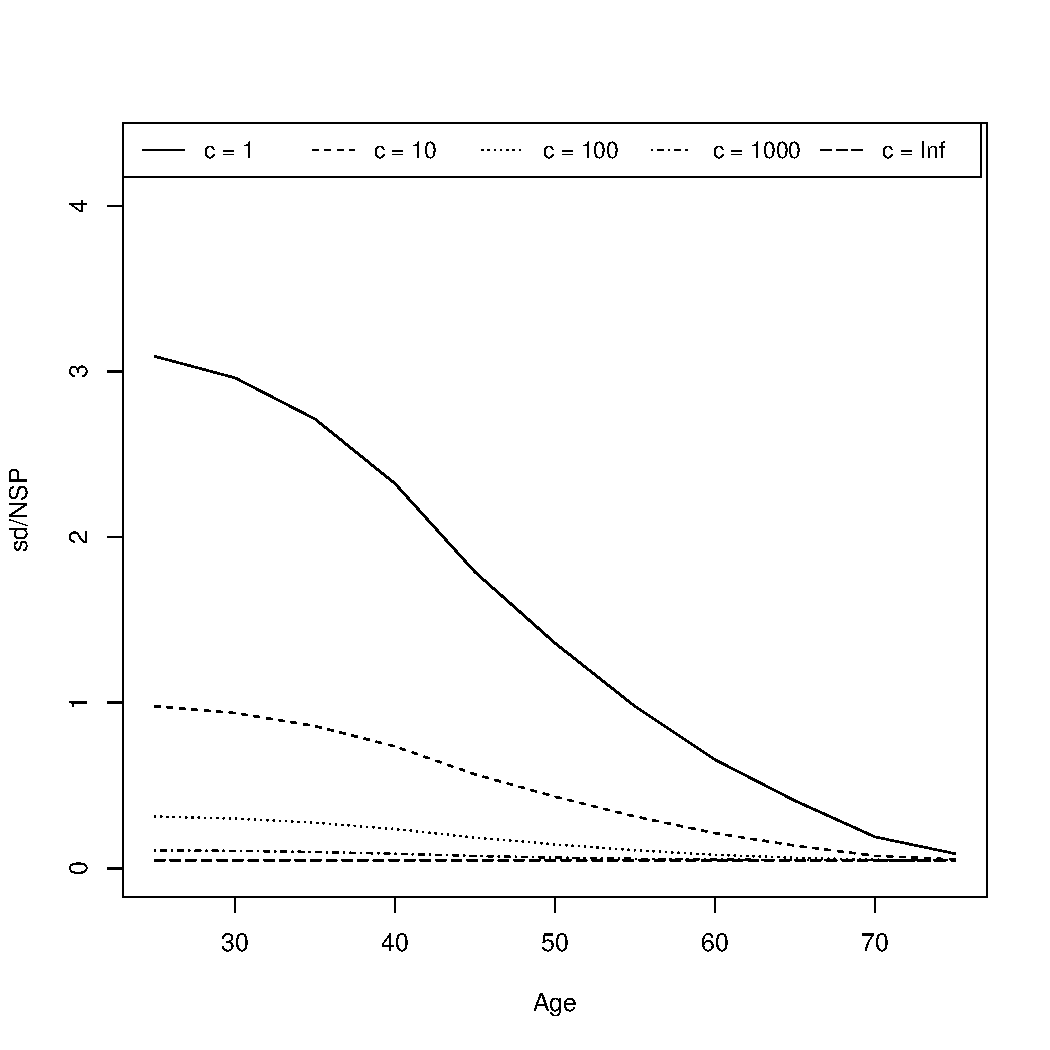
\includegraphics[width=1.0\textwidth]{images/portfolioRiskMale5}
\end{center}
\subcaption{$n$ = 5 (Male)}
\end{minipage}
\begin{minipage}[b]{0.55\textwidth}
\begin{center}
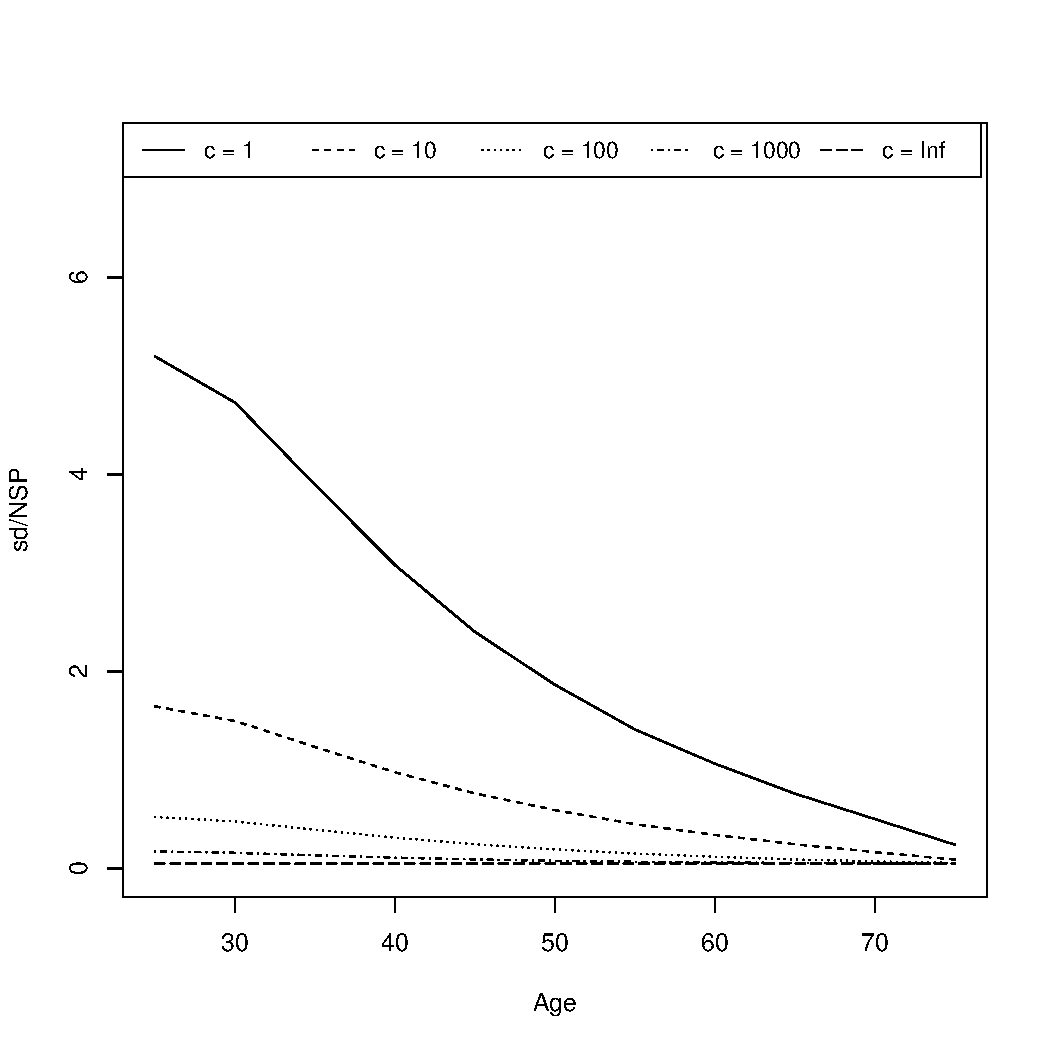
\includegraphics[width=1.0\textwidth]{images/portfolioRiskFemale5}
\end{center}
\subcaption{$n$ = 5 (Female)}
\end{minipage}
}
\vspace{-8mm}
\centerline{
\begin{minipage}[b]{0.55\textwidth}
\begin{center}
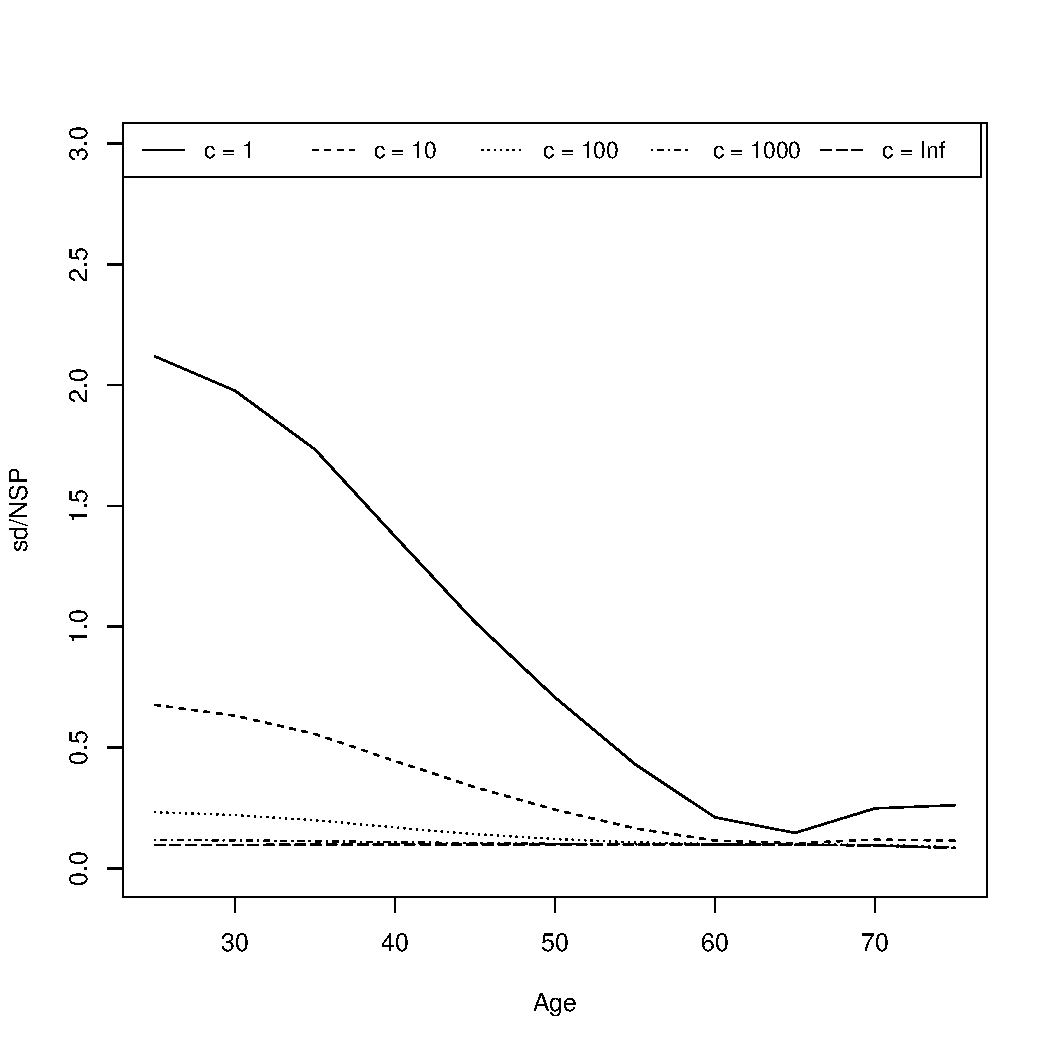
\includegraphics[width=1.0\textwidth]{images/portfolioRiskMale10}
\end{center}
\subcaption{$n$ = 10 (Male)}
\end{minipage}
\begin{minipage}[b]{0.55\textwidth}
\begin{center}
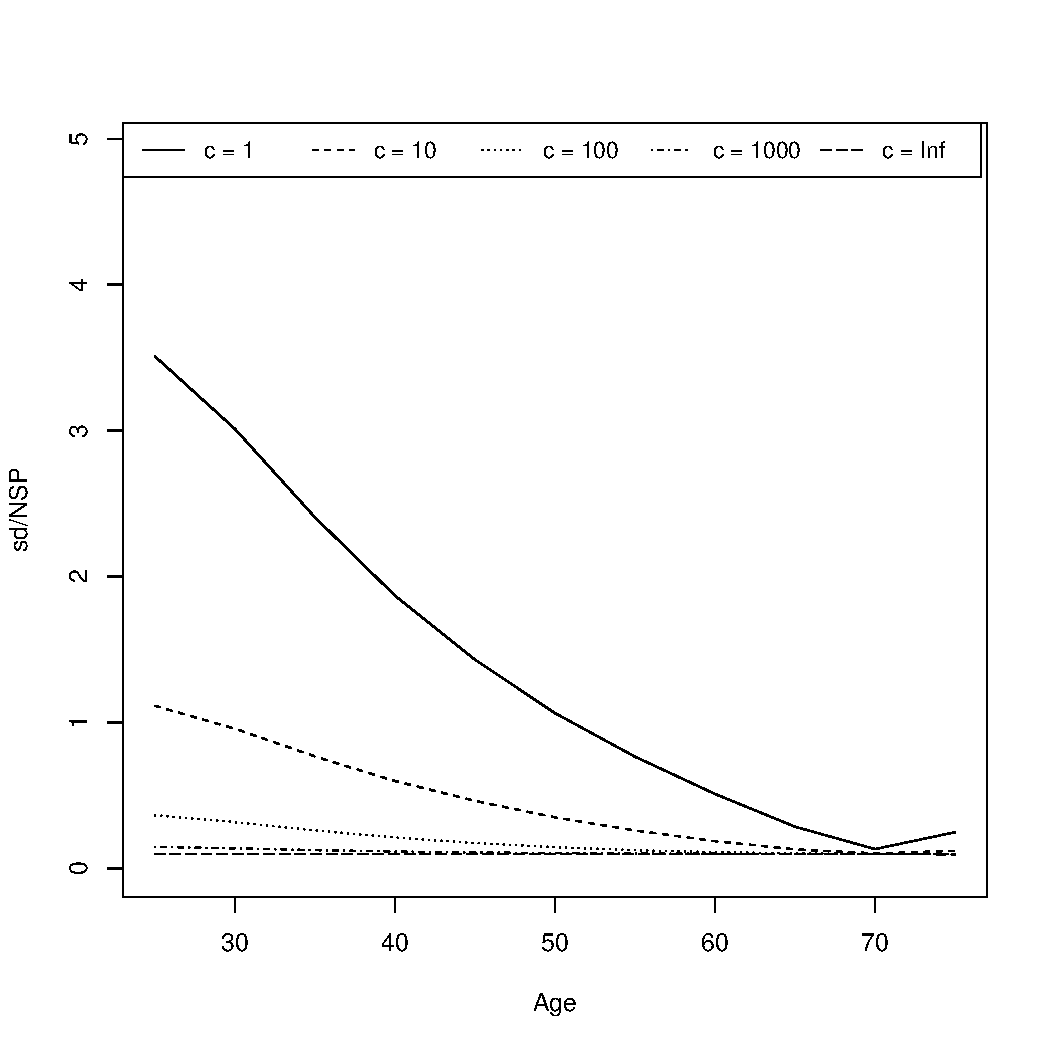
\includegraphics[width=1.0\textwidth]{images/portfolioRiskFemale10}
\end{center}
\subcaption{$n$ = 10 (Female)}
\end{minipage}
}
\end{center}
\caption{Standard deviation per dollar premium for $c$ identical $n$-year endowment contracts}
\label{fig:portfoliosd}
\end{figure}

The question addressed here is -- how many contracts are needed to remove the insurance risk through pooling? We can see that to get close to the limiting standard deviation (i.e. no insurance risk), around 100 policies are needed in most cases.

While we may not have 100 policies for a specific age and term, the curve of deaths is relatively flat between 20 and 40. Therefore, if we have many policyholders with similar ages and terms, we should be able to eliminate most of the insurance risk. 

It is harder to eliminate the insurance risk for older ages (since the curve of deaths is not flat between 60 to 70), so the ages need to be very close together for pooling to work. However, the death benefit is also much smaller for older ages in comparison to the premium. So the insurance risk for these policies is not as concerning to us as the insurance risk for the younger ages.

Note that the limiting portfolio still has a positive standard deviation per dollar premium. This is due to the investment risk, which is not removed through pooling.

\subsection{Groups of policies}

To obtain some results on the investment and insurance risk for a product, an illustrative portfolio of 2000 contracts was constructed as follows:

\begin{itemize}
\item The age distribution follows the distribution shown in Appendix A.3 with policyholder ages ranging from 25 to 75 (midpoint of each age interval used).
\item 1/2 of the endowment contracts have term $n = 5$ and 1/2 have term $n = 10$.
\item 1/2 of the contracts are issued to males and 1/2 of the contracts are issued to females.
\item 4/5 of the contracts have death benefit \$500,000 and 1/5 of the contracts have death benefit \$5,000,000.
\end{itemize}

The illustrative portfolio can be found in Appendix A.5.

\subsection{Investment and insurance risk}

The net single premium, insurance risk, investment risk and standard deviation per policy for the Illustrative Portfolio are shown in Table \ref{tab:risktable}.

% latex table generated in R 3.3.1 by xtable 1.8-2 package
% Fri Apr 07 09:21:25 2017
\begin{table}[ht]
\centering
\begingroup\small
\begin{tabular}{lrrrrr}
  \hline
Num Policies & NSP & Ins Risk & Inv Risk & SD & SD/NSP \\ 
  \hline
200 & 281.86 & 447.78 & 460.08 & 30.13 & 0.1069 \\ 
  1000 & 281.86 & 89.56 & 460.08 & 23.44 & 0.0832 \\ 
  2000 & 281.86 & 44.78 & 460.08 & 22.47 & 0.0797 \\ 
  4000 & 281.86 & 22.39 & 460.08 & 21.97 & 0.0779 \\ 
  20000 & 281.86 & 4.48 & 460.08 & 21.55 & 0.0765 \\ 
  $\infty$ & 281.86 & 0.00 & 460.08 & 21.45 & 0.0761 \\ 
   \hline
\end{tabular}
\endgroup
\caption{Investment and Insurance Risk for the Illustrative Portfolio} 
\label{tab:risktable}
\end{table}



We can see that, for 200 policies, the insurance risk is about the same size as the investment risk, whereas for 2000 policies, the insurance risk has decreased significantly as a result of pooling. It would be possible to decrease the insurance risk even more by selling more policies. However, this product is targeted to wealthy investors and there is a limited number of wealthy people. So selling more policies is unlikely to be an option.

Decreasing the insurance risk more isn't much of a concern though. At $c = 2000$ policyholders, the insurance risk is only 9\% of the total risk, so it's already mostly mitigated. Even the insurance risk of 5 year policies, which is significant for a single policyholder (i.e. see Figure \ref{fig:sdendow}) is mostly mitigated.

Our attention now turns to the investment risk. This is much higher for 10 year policies than for 5 year policies. The reason for this is because the standard deviation of the present value is higher for a 10 year investment than for a 5 year investment (i.e. see Figure \ref{fig:pvvar}). Therefore, obvious way to decrease the investment risk is to sell shorter policies. However, the issue with this is that investors may have a preference for longer term policies as these offer a higher return upon survival (i.e. see Table \ref{tab:returnTable}).

In fact, the investment risk is highest for policies for long term contracts with large survival benefits (i.e. those issued to older ages). But these policyholders also pay a much higher premium (see Table \ref{tab:faceAmountTable}) so the standard deviation per dollar premium is not necessarily higher for these policyholders.

\section{Conclusion}

The main findings of this support are now summarized.

Firstly, the standard deviation per dollar premium is highest for short term contracts issued to younger ages since these policies have a significantly larger death benefit than survival benefit. The majority of this risk is coming from the insurance risk. However, with a portfolio size of $c = 2000$ this insurance risk can be mostly mitigated through pooling.

On the other hand, the investment risk is higher for long term policies with large survival benefits. This risk cannot be removed through pooling. It may be possible to hedge this risk, but this would be expensive and we would have to charge a higher premium to make up for this cost, making the product less competitive.

The standard deviation in comparison to the premium collected was found to be around 8\% for a portfolio size of $c = 2000$. If management believes this is acceptable, this product could be sold. If this is still too high, the simplest thing to do would be to sell shorter term contracts (if investors are still willing to buy these).

\newpage

\begin{appendices}

\section{Additional Tables and Figures}

\subsection{OU Process using returns from 1991 to 2017}

\begin{figure}[ht]
\begin{center}
\vspace{-12.5mm}
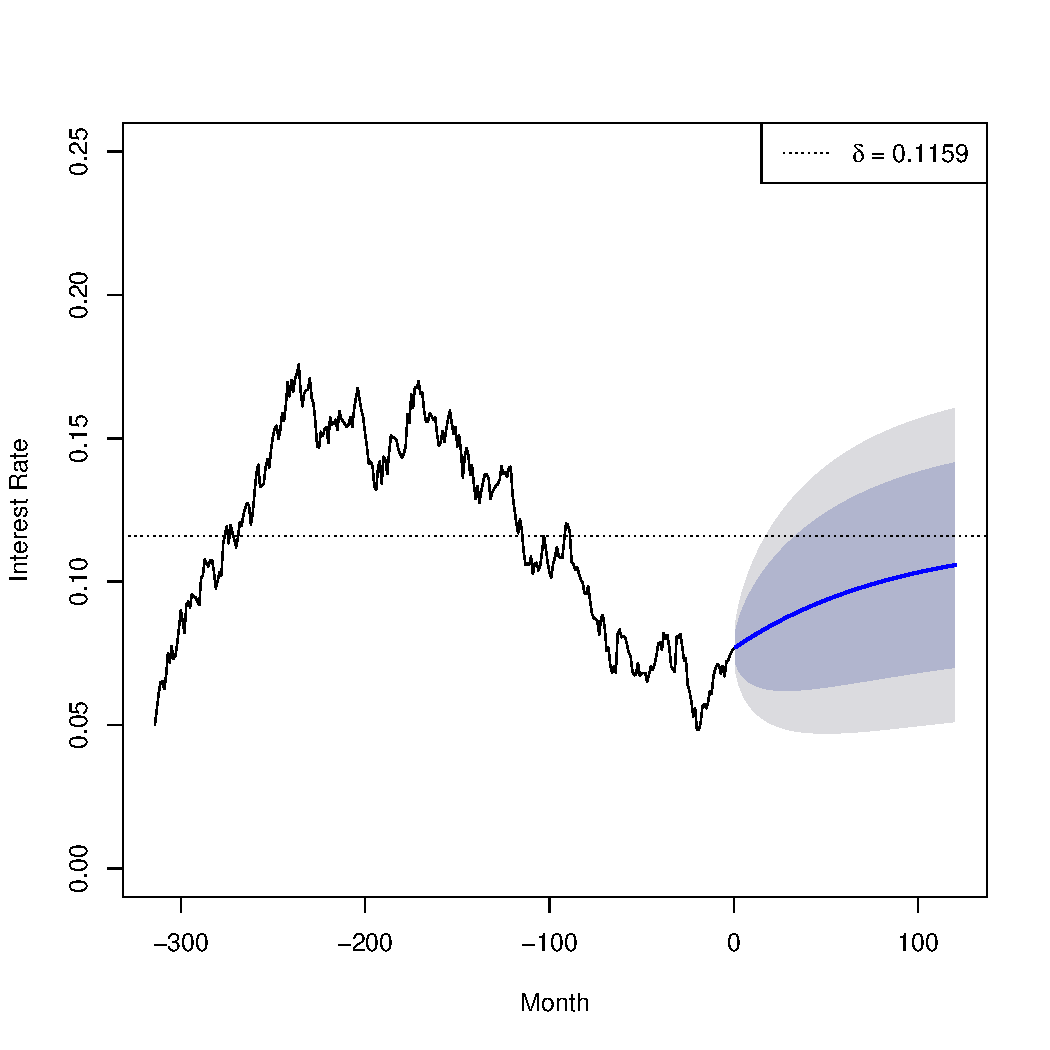
\includegraphics[width=0.65\textwidth]{images/arforecast1991}
\end{center}
\vspace{-2.5mm}
\caption{Expected interest rate over next 10 years using an OU process with $\delta_{0} = 0.0767$, $\delta = 0.1159$, $\alpha = 0.1352$ and $\sigma = 0.01501$. The 80\% and 95\% confidence intervals are shown.}
\label{fig:ouforecast1991}
\end{figure}

\subsection{Risk for Alternative Interest Rate Models}

\subsubsection{OU Process using returns from 1991 to 2017}

The results of Section 4.2 are recalculated here using the OU process  from Appendix A.1. The net single premium is lower as a result of the higher interest rate, but the standard deviation is higher as a result of the higher investment volatility.

\input{tables/risktable1991}

\subsubsection{Covariance equivalent AR(1) Process}

The covariance equivalent AR(1) process is $\phi = 0.77835$, $\sigma = 0.01289$, $\delta = 0.05$ and $\delta_{0} = 0.0767$. Using this (discrete) process gives similar results to using a OU process (i.e. Table \ref{tab:risktableAR1} is similar to Table \ref{tab:risktable}) as expected.

\input{tables/risktableAR1}

\subsubsection{Deterministic Interest Rate}

As expected, there is no investment risk when a deterministic interest rate is used. The standard deviation for the portfolio goes to 0 as the number of policies increases. Since $\delta_{0} > \delta$ the expected interest rate is higher when an OU process is used. This makes the $NSP$ lower for an OU process.

\input{tables/risktableDeterm}

\newpage

\subsection{Portfolio age distribution}

\begin{figure}[!htpb]
\begin{center}
\vspace{-10mm}
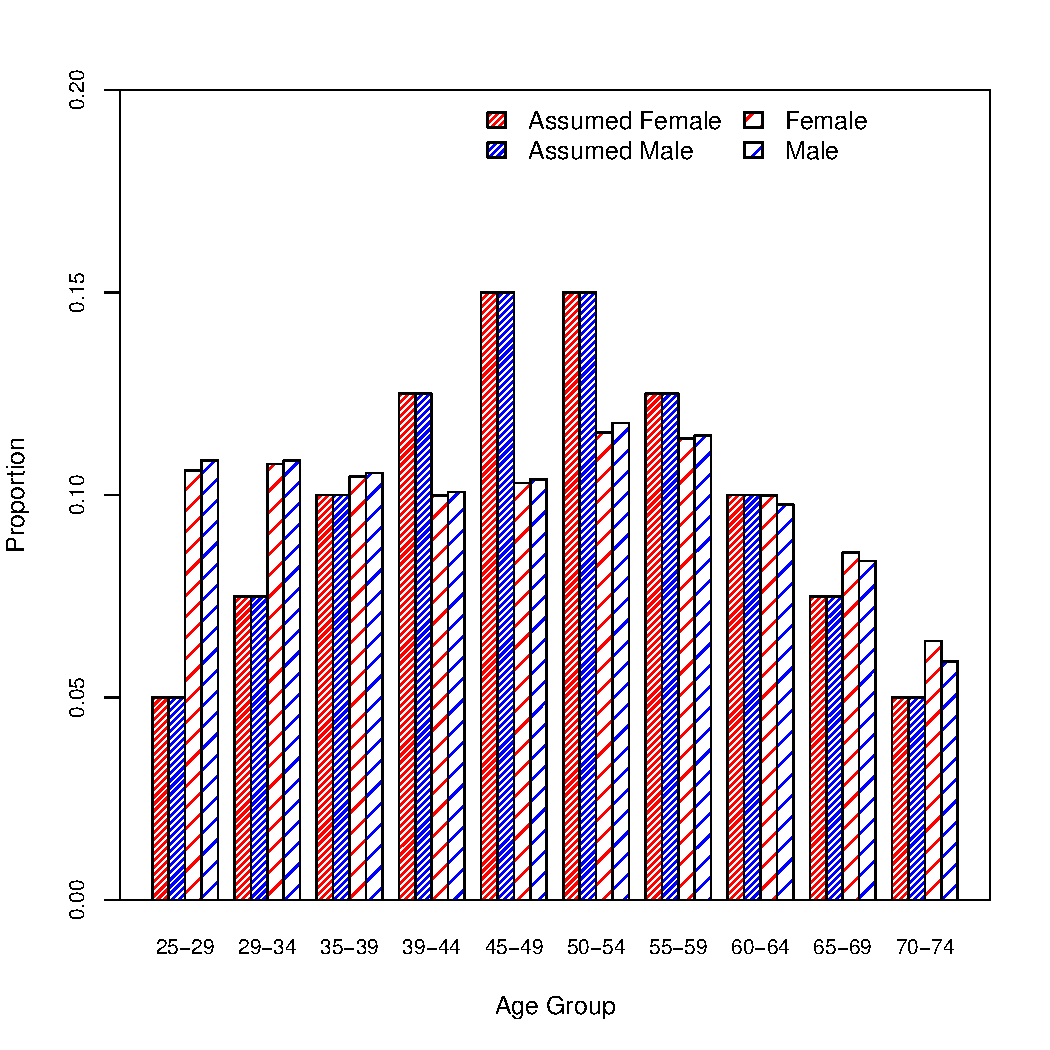
\includegraphics[width=0.7\textwidth]{images/agedistribution}
\end{center}
\vspace{-3mm}
\caption{Assumed age distribution alongside 2016 Canadian population table}
\label{fig:agedistribution}
\end{figure}

\subsection{EPV for term and pure endowment contracts}

% latex table generated in R 3.3.1 by xtable 1.8-2 package
% Fri Apr 07 09:37:02 2017
\begin{table}[!htpb]
\centering
\begingroup\small
\begin{tabular}{|l|rrrr|rrrr|}
  \hline
& \multicolumn{4}{c|}{5-year} & \multicolumn{4}{c|}{10-year} \\
 & \multicolumn{2}{c}{Male} & \multicolumn{2}{c|}{Female} & \multicolumn{2}{c}{Male} & \multicolumn{2}{c|}{Female} \\
 \hline
Age & $E$[Term] & $E$[Pure] & $E$[Term] & $E$[Pure] & $E$[Term] & $E$[Pure] & $E$[Term] & $E$[Pure] \\ 
  \hline
25 & 0.0052 & 0.7183 & 0.0019 & 0.7212 & 0.0094 & 0.5462 & 0.0036 & 0.5507 \\ 
  30 & 0.0056 & 0.7179 & 0.0023 & 0.7208 & 0.0105 & 0.5452 & 0.0047 & 0.5497 \\ 
  35 & 0.0066 & 0.7170 & 0.0033 & 0.7199 & 0.0132 & 0.5430 & 0.0072 & 0.5477 \\ 
  40 & 0.0088 & 0.7150 & 0.0052 & 0.7182 & 0.0193 & 0.5379 & 0.0113 & 0.5443 \\ 
  45 & 0.0141 & 0.7103 & 0.0082 & 0.7155 & 0.0307 & 0.5287 & 0.0180 & 0.5390 \\ 
  50 & 0.0225 & 0.7027 & 0.0131 & 0.7111 & 0.0499 & 0.5132 & 0.0288 & 0.5302 \\ 
  55 & 0.0374 & 0.6894 & 0.0212 & 0.7039 & 0.0823 & 0.4872 & 0.0456 & 0.5169 \\ 
  60 & 0.0624 & 0.6672 & 0.0332 & 0.6932 & 0.1303 & 0.4495 & 0.0713 & 0.4963 \\ 
  65 & 0.0977 & 0.6360 & 0.0527 & 0.6759 & 0.1958 & 0.3983 & 0.1107 & 0.4650 \\ 
  70 & 0.1482 & 0.5912 & 0.0824 & 0.6495 & 0.2871 & 0.3276 & 0.1733 & 0.4150 \\ 
  75 & 0.2259 & 0.5231 & 0.1344 & 0.6033 & 0.4052 & 0.2395 & 0.2705 & 0.3390 \\ 
   \hline
\end{tabular}
\endgroup
\caption{$EPV$ for term and pure endowment contracts used in pricing} 
\end{table}



\newpage

\subsection{Illustrative Portfolio}

% latex table generated in R 3.3.1 by xtable 1.8-2 package
% Fri Apr 07 09:38:27 2017
\begin{table}[!htpb]
\centering
\begingroup\small
\begin{tabular}{lrrrrr|lrrrrr}
  \hline
Group & Size & Age & Gender & $n$ & $d$ & Group & Size & Age & Gender & $n$ & $d$ \\ 
  \hline
1 & 20 & 27 & Male & 5 & 500 & 41 & 20 & 27 & Male & 10 & 500 \\ 
  2 & 30 & 32 & Male & 5 & 500 & 42 & 30 & 32 & Male & 10 & 500 \\ 
  3 & 40 & 37 & Male & 5 & 500 & 43 & 40 & 37 & Male & 10 & 500 \\ 
  4 & 50 & 42 & Male & 5 & 500 & 44 & 50 & 42 & Male & 10 & 500 \\ 
  5 & 60 & 47 & Male & 5 & 500 & 45 & 60 & 47 & Male & 10 & 500 \\ 
  6 & 60 & 52 & Male & 5 & 500 & 46 & 60 & 52 & Male & 10 & 500 \\ 
  7 & 50 & 57 & Male & 5 & 500 & 47 & 50 & 57 & Male & 10 & 500 \\ 
  8 & 40 & 62 & Male & 5 & 500 & 48 & 40 & 62 & Male & 10 & 500 \\ 
  9 & 30 & 67 & Male & 5 & 500 & 49 & 30 & 67 & Male & 10 & 500 \\ 
  10 & 20 & 72 & Male & 5 & 500 & 50 & 20 & 72 & Male & 10 & 500 \\ 
  11 & 20 & 27 & Female & 5 & 500 & 51 & 20 & 27 & Female & 10 & 500 \\ 
  12 & 30 & 32 & Female & 5 & 500 & 52 & 30 & 32 & Female & 10 & 500 \\ 
  13 & 40 & 37 & Female & 5 & 500 & 53 & 40 & 37 & Female & 10 & 500 \\ 
  14 & 50 & 42 & Female & 5 & 500 & 54 & 50 & 42 & Female & 10 & 500 \\ 
  15 & 60 & 47 & Female & 5 & 500 & 55 & 60 & 47 & Female & 10 & 500 \\ 
  16 & 60 & 52 & Female & 5 & 500 & 56 & 60 & 52 & Female & 10 & 500 \\ 
  17 & 50 & 57 & Female & 5 & 500 & 57 & 50 & 57 & Female & 10 & 500 \\ 
  18 & 40 & 62 & Female & 5 & 500 & 58 & 40 & 62 & Female & 10 & 500 \\ 
  19 & 30 & 67 & Female & 5 & 500 & 59 & 30 & 67 & Female & 10 & 500 \\ 
  20 & 20 & 72 & Female & 5 & 500 & 60 & 20 & 72 & Female & 10 & 500 \\ 
  21 & 5 & 27 & Male & 5 & 5000 & 61 & 5 & 27 & Male & 10 & 5000 \\ 
  22 & 8 & 32 & Male & 5 & 5000 & 62 & 8 & 32 & Male & 10 & 5000 \\ 
  23 & 10 & 37 & Male & 5 & 5000 & 63 & 10 & 37 & Male & 10 & 5000 \\ 
  24 & 12 & 42 & Male & 5 & 5000 & 64 & 12 & 42 & Male & 10 & 5000 \\ 
  25 & 15 & 47 & Male & 5 & 5000 & 65 & 15 & 47 & Male & 10 & 5000 \\ 
  26 & 15 & 52 & Male & 5 & 5000 & 66 & 15 & 52 & Male & 10 & 5000 \\ 
  27 & 12 & 57 & Male & 5 & 5000 & 67 & 12 & 57 & Male & 10 & 5000 \\ 
  28 & 10 & 62 & Male & 5 & 5000 & 68 & 10 & 62 & Male & 10 & 5000 \\ 
  29 & 8 & 67 & Male & 5 & 5000 & 69 & 8 & 67 & Male & 10 & 5000 \\ 
  30 & 5 & 72 & Male & 5 & 5000 & 70 & 5 & 72 & Male & 10 & 5000 \\ 
  31 & 5 & 27 & Female & 5 & 5000 & 71 & 5 & 27 & Female & 10 & 5000 \\ 
  32 & 8 & 32 & Female & 5 & 5000 & 72 & 8 & 32 & Female & 10 & 5000 \\ 
  33 & 10 & 37 & Female & 5 & 5000 & 73 & 10 & 37 & Female & 10 & 5000 \\ 
  34 & 12 & 42 & Female & 5 & 5000 & 74 & 12 & 42 & Female & 10 & 5000 \\ 
  35 & 15 & 47 & Female & 5 & 5000 & 75 & 15 & 47 & Female & 10 & 5000 \\ 
  36 & 15 & 52 & Female & 5 & 5000 & 76 & 15 & 52 & Female & 10 & 5000 \\ 
  37 & 12 & 57 & Female & 5 & 5000 & 77 & 12 & 57 & Female & 10 & 5000 \\ 
  38 & 10 & 62 & Female & 5 & 5000 & 78 & 10 & 62 & Female & 10 & 5000 \\ 
  39 & 8 & 67 & Female & 5 & 5000 & 79 & 8 & 67 & Female & 10 & 5000 \\ 
  40 & 5 & 72 & Female & 5 & 5000 & 80 & 5 & 72 & Female & 10 & 5000 \\ 
   \hline
\end{tabular}
\endgroup
\caption{The illustrative portfolio used. The endowment benefit for each group is calculated using Equation 1.} 
\label{tab:groupstable}
\end{table}



\end{appendices}

\linespread{1.5}

\bibliography{sources}

\end{document}